\documentclass[11pt]{article}
\usepackage[utf8]{inputenc}
\usepackage[T1]{fontenc}
\usepackage{geometry, tikz, xcolor, enumitem, ragged2e}
\geometry{a4paper, margin=1.5cm}

\begin{document}

\begin{center}
\Large \textbf{\textcolor{blue!60!black}{Atividade: Matemática – Progressão Geométrica (PG)}}\\[0.3cm]
\large Professor: Jefferson
\end{center}

\vspace{0.3cm}
\large Nome: \underline{\hspace{8cm}} \quad Turma: \underline{\hspace{3cm}}

\vspace{0.5cm}

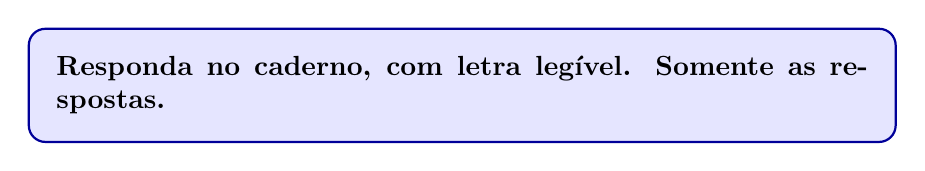
\begin{tikzpicture}
\node[rectangle, fill=blue!10, rounded corners=6pt, inner sep=10pt, draw=blue!60!black, thick]{
\begin{minipage}{0.85\linewidth}
\textbf{Responda no caderno, com letra legível. Somente as respostas.}
\end{minipage}
};
\end{tikzpicture}

\vspace{0.6cm}

\begin{enumerate}

\item Explique, com suas palavras, o que caracteriza uma sequência numérica como Progressão Geométrica.

\item O que chamamos de \textbf{razão} de uma PG? Descreva como ela pode ser encontrada.

\item Qual a diferença entre uma PG crescente, decrescente e constante? Cite um exemplo de cada.

\item Na fórmula do termo geral $a_n = a_1 \cdot q^{\,n-1}$, explique o significado de cada elemento ($a_n$, $a_1$, $n$, $q$).

\item Em uma PG, se conhecemos dois termos não consecutivos, como podemos descobrir a razão? Descreva o procedimento.

\item Por que a soma dos termos de uma PG finita pode ser calculada usando a fórmula $S_n = a_1 \frac{q^n - 1}{q-1}$ (para $q \neq 1$)? Explique o raciocínio.

\item Cite pelo menos duas situações do cotidiano em que uma Progressão Geométrica pode aparecer.

\item Explique por que toda PG possui comportamento de crescimento ou decrescimento exponencial, e não linear.

\item Calcule o 6º termo da PG: $2, 4, 8, 16, \dots$

\item Uma PG tem primeiro termo $a_1 = 3$ e razão $q = 2$. Determine o 5º termo.

\item Encontre a soma dos 8 primeiros termos da PG: $1, 3, 9, 27, \dots$

\item Se o 3º termo de uma PG é 24 e o 6º termo é 192, determine o primeiro termo e a razão.
\end{enumerate}

\vspace{1cm}
\textbf{\Large Gabarito (Respostas-modelo)}

\begin{enumerate}

\item Uma sequência é uma PG quando a razão entre um termo e o termo anterior é sempre constante.

\item A razão $q$ é o valor que se multiplica para passar de um termo ao próximo. Calcula-se fazendo $q = \frac{a_n}{a_{n-1}}$.

\item PG crescente: $q>1$ (ex.: $2, 4, 8, 16,\dots$) \\
PG decrescente: $0<q<1$ (ex.: $81, 27, 9, 3,\dots$) \\
PG constante: $q=1$ (ex.: $5, 5, 5, 5,\dots$)

\item $a_n$ é o termo desejado; $a_1$ é o primeiro termo; $n$ é a posição do termo; $q$ é a razão da PG.

\item Podemos usar $a_n = a_1 \cdot q^{n-1}$ para montar duas equações e resolver para $q$ usando radiciação ou divisão.

\item A soma de uma PG finita pode ser reorganizada e fatorada de forma que se obtenha a fórmula $S_n = a_1 \frac{q^n - 1}{q-1}$, pois cada termo é múltiplo constante do anterior.

\item Exemplos: crescimento populacional, juros compostos, duplicação de vírus, investimentos que rendem percentualmente.

\item Porque em uma PG sempre multiplicamos por um valor constante a cada passo, gerando crescimento ou decrescimento exponencial.

\item $a_6 = 2 \cdot 2^{6-1} = 2 \cdot 32 = 64$

\item $a_5 = 3 \cdot 2^{5-1} = 3 \cdot 16 = 48$

\item $S_8 = 1 \cdot \frac{3^8 - 1}{3-1} = \frac{6561 - 1}{2} = \frac{6560}{2} = 3280$

\item $a_3 = a_1 \cdot q^2 = 24 \Rightarrow a_1 \cdot q^2 = 24$ \\
$a_6 = a_1 \cdot q^5 = 192 \Rightarrow a_1 \cdot q^5 = 192$ \\
Dividindo: $q^3 = 192/24 = 8 \Rightarrow q = 2$ \\
Então $a_1 \cdot 2^2 = 24 \Rightarrow a_1 = 6$
\end{enumerate}

\end{document}

